
% Amazon Silk vs Google Chrome

%1
\newcommand{\qSilkMobileDevices}{
\begin{ClosedQuestion}
	When comparing Amazon Silk with Google Chrome in the context of mobile devices

    \optionA{Amazon Silk is more convenient for mobile devices because it does most of the computation in the cloud.}
    \optionB{Google Chrome is more convenient for mobile devices because it has an optimized network stack that runs in any kind device.}
    \optionC{Amazon Silk is more convenient for mobile devices because it customizes the number of threads that run in the device.}
    \optionD{Google Chrome is more convenient for mobile devices because content delivery is optimized.}
 \putOptions
\end{ClosedQuestion}
}

%2
\newcommand{\qSilkPredictor}{
\begin{ClosedQuestion}
	When comparing Amazon Silk with Google Chrome in the context of the prediction of pages the user is going to access
	
    \optionA{Amazon Silk predicts accesses based on the information gathered for all Silk users.}
    \optionB{Google Chrome uses a usability maintain system model tactic.}
    \optionC{Amazon Silk predictions are constrained by the amount of information it can store about each user access.}
    \optionD{Google Chrome predictions do not require storage in the client-side.}
 \putOptions
\end{ClosedQuestion}
}

%3
\newcommand{\qSilkCaching}{
\begin{ClosedQuestion}
	When comparing Amazon Silk with Google Chrome  

    \optionA{Amazon Silk explicitly caches pages on the browser to optimize accesses.}
    \optionB{Google Chrome predictor takes into consideration the amount of available cache.}
    \optionC{Amazon Silk cache is not shared between different users of the service to support confidentiality.}
    \optionD{Google Chrome cache is shared among the different users of a desktop machine.}
 \putOptions
\end{ClosedQuestion}
}

%4
\newcommand{\qSilkConnections}{
\begin{ClosedQuestion}
	When comparing Amazon Silk with Google Chrome  
	
    \optionA{In Amazon Silk a request for a web page corresponds to a peer-to-peer interaction between all the web components containing the resources.}
    \optionB{In Google Chrome a request for a web page is accomplished by a single access to the internet.}
    \optionC{In Amazon Silk a request for a web page corresponds to requesting a service from the amazon cloud.}
    \optionD{In Google Chrome a request for a web page aggregates the page on the background before it is sent to the client.}
 \putOptions
\end{ClosedQuestion}
}


% ThousandParsec views

%5 
\newcommand{\qThousandParsecAI}{
\begin{ClosedQuestion}
	Consider the architectural views for the ThousandParsec system. The following diagram depicts a fragment of a proposal for the decomposition view of the system. The AI players should be described
	
	\centering
	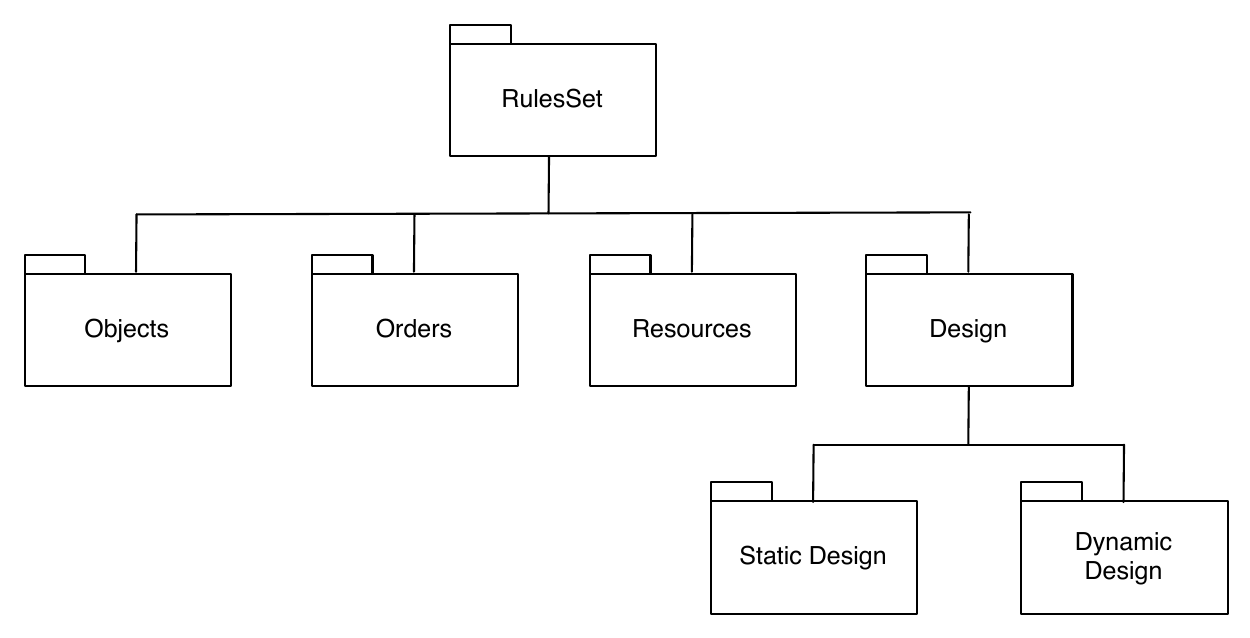
\includegraphics[width=100mm]{x-ThousandParsec-ruleset}

    \optionA{As a specialization of the RulesSet module.}
    \optionB{As a submodule of the RulesSet module.}
    \optionC{As a module but not included in the RulesSet subtree.}
    \optionD{As a specialization of the Design module.}
 \putOptions
\end{ClosedQuestion}
}

%6 
\newcommand{\qThousandParsecModule}{
\begin{ClosedQuestion}
	Consider the architectural views for the ThousandParsec system. The following diagram depicts a fragment of a proposal for the decomposition view of the system. The ThousandParsec protocol
	
	\centering
	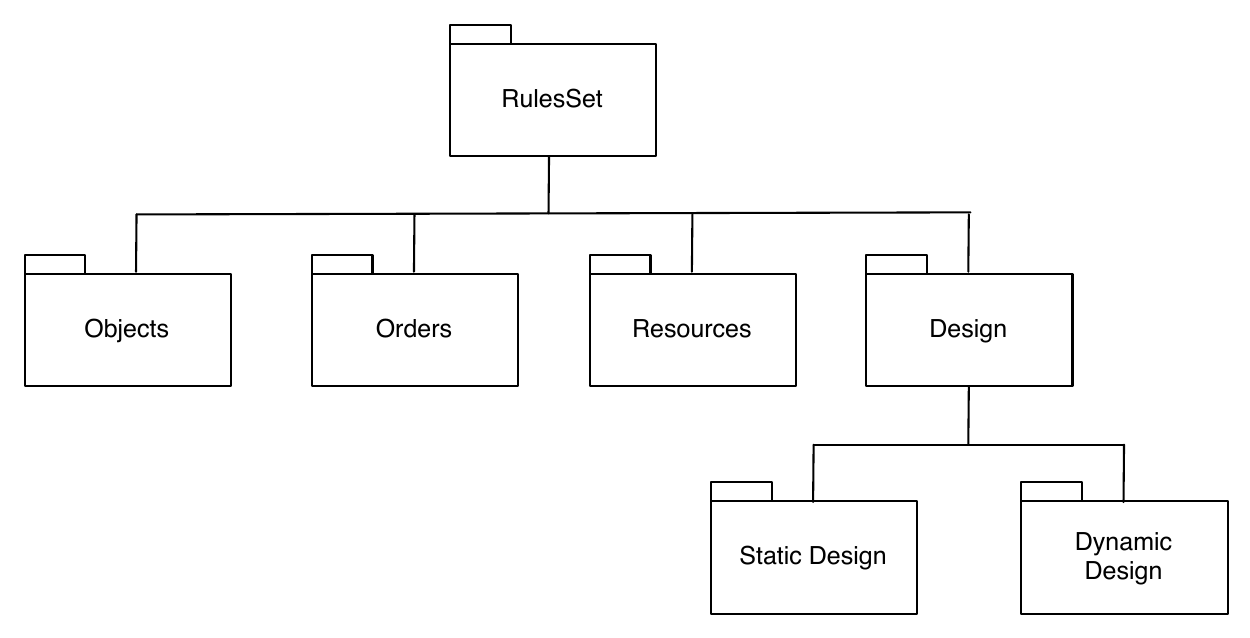
\includegraphics[width=100mm]{x-ThousandParsec-ruleset}

    \optionA{Should be described as a submodule of the RulesSet module.}
    \optionB{Should be described as a submodule of but not included in the RulesSet subtree.}
    \optionC{Should be described as a submodule of the Design module.}
    \optionD{Should not be described as a module because it is a component.}
 \putOptions
\end{ClosedQuestion}
}

%7 
\newcommand{\qThousandParsecTPConnector}{
\begin{ClosedQuestion}
	Consider the architectural views for the ThousandParsec system. The following diagram depicts a proposal of application-specific types for the architectural components, where the names of the ports are missing. Between the GameClient and GameServer components
	
	\centering
	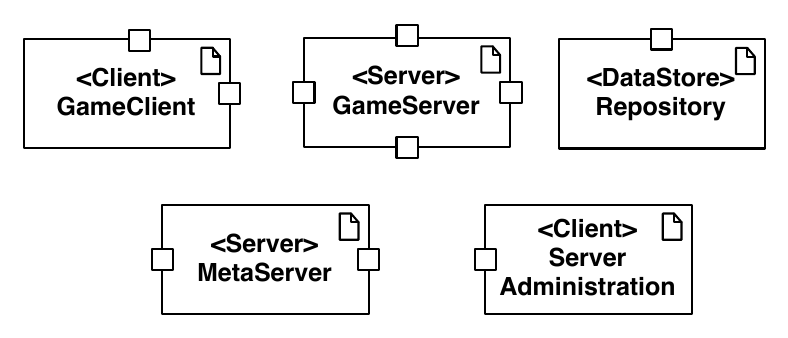
\includegraphics[width=80mm]{x-ThousandParsec-cc}

    \optionA{There is a ThousandParsec connector.}
    \optionB{There is a Request/Reply connector.}
    \optionC{There is a ThousandParsec connector which can be decomposed into a set of components and Request/Reply connectors.}
    \optionD{There is an EventBus connector.}
 \putOptions
\end{ClosedQuestion}
}

%8 
\newcommand{\qThousandParsecReadWriteConnector}{
\begin{ClosedQuestion}
	Consider the architectural views for the ThousandParsec system. The following diagram depicts a proposal of application-specific types for the architectural components, where the names of the ports are missing. Between the GameServer and Repository component
	
	\centering
	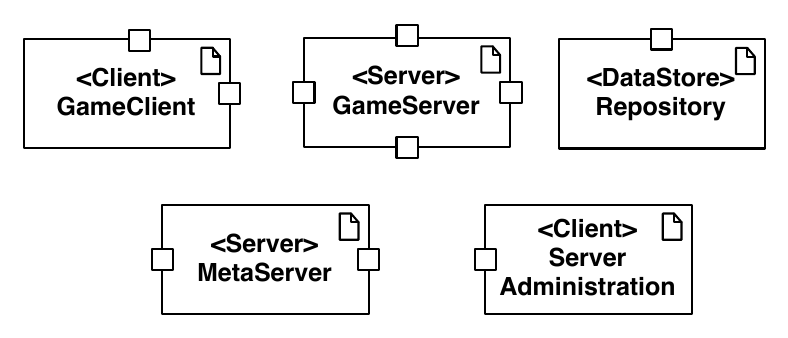
\includegraphics[width=80mm]{x-ThousandParsec-cc}

    \optionA{There is a ThousandParsec connector.}
    \optionB{There is a Read/Write connector which encapsulates a redundant Repository.}
    \optionC{There is a Read/Write connector which guarantees that players turns are not lost.}
    \optionD{There is a Read/Write connector which guarantees that only the turns of the last two players may be lost.}
 \putOptions
\end{ClosedQuestion}
}


% The architecture of OrderPad

%9
\newcommand{\qOrderPadPortability}{
\begin{ClosedQuestion}
	Consider the architecture of the Morrison's OrderPad. The decision between the use of a Native application or HTML5 on the implementation of the client in the Pad
	
    \optionA{Was taken because HTML5 provides better portability qualities.}
    \optionB{Was taken because Native applications provide better modifiability qualities.}
    \optionC{Was taken because HTML5 provides better usability qualities.}
    \optionD{Was taken because Native application provide better support for working offline.}
 \putOptions
\end{ClosedQuestion}
}

%10
\newcommand{\qOrderPadReliability}{
\begin{ClosedQuestion}
	Consider the architecture of the Morrison's OrderPad. The connector between the client component, executing in the Pad, and the server component, executing in the OrderPadDatabase
	
    \optionA{Supports asynchronous communication to deal with disconnected mode.}
    \optionB{Implements an event bus that allows the server to inform the client about new order recommendations.}
    \optionC{May loose some of the changes done on the client component.}
    \optionD{Has reduced reliability qualities.}
 \putOptions
\end{ClosedQuestion}
}

%11
\newcommand{\qOrderPadMainframeConnector}{
\begin{ClosedQuestion}
	Consider the architecture of the Morrison's OrderPad. The final interaction between the OrderPadDatabase component and Mainframe component is supported by 
	
    \optionA{Two distinct unidirectional connectors.}
    \optionB{A single bidirectional connector.}
    \optionC{Three distinct unidirectional connectors.}
    \optionD{A single unidirectional connector.}
 \putOptions
\end{ClosedQuestion}
}

%12
\newcommand{\qOrderPadIterative}{
\begin{ClosedQuestion}
	Consider the architecture of the Morrison's OrderPad. In the description of the system can be read:
	
	\begin{quote}
		One of these was using a file-transfer to send data to the mainframe rather than MQ, which wouldn't perform well once many stores were active.
	\end{quote}
	
	This approach means that
	
    \optionA{Performance was traded for easy of development.}
    \optionB{An iterative development was followed, which allowed more time to develop a connector with good performance in the latter stages of the project.}
    \optionC{Performance was traded for the modifiability quality.}
    \optionD{An incremental development was followed, which allowed to have the system in production without being necessary to export all the information to the mainframe.}
 \putOptions
\end{ClosedQuestion}
}


% SocialCalc Views

%13
\newcommand{\qSocialCalcRemoteCursor}{
\begin{ClosedQuestion}
	Consider the architectural views for the SocialCalc system. The following diagram depicts a proposal for a component-and-connector view of the client Spreadsheet. It can be read in the case description: \emph{A simple improvement is for each client to broadcast its cursor position to other users, so everyone can see which cells are being worked on.}
	
	\centering
	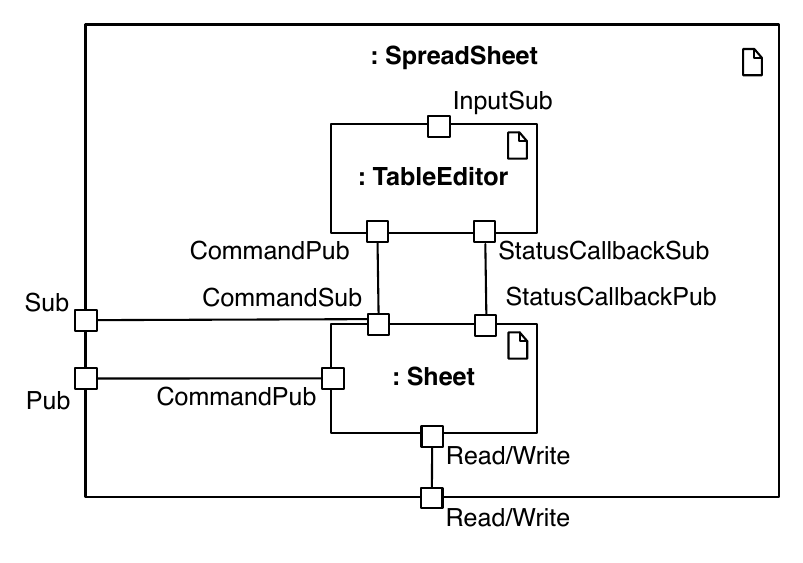
\includegraphics[width=80mm]{x-SocialCalc-cc-client}

    \optionA{The \textsc{: TableEditor} broadcasts the cursor position through the \textsc{: Sheet}.}
    \optionB{An interface delegation is missing in the picture to represent the \textsc{: TableEditor} broadcasting the cursor position through the \textsc{Pub} port.}
    \optionC{The \textsc{: Sheet} broadcasts the cursor position through the \textsc{Pub} port.}
    \optionD{The \textsc{: TableEditor} broadcasts the cursor position through its \textsc{: StatusCallback} port.}
 \putOptions
\end{ClosedQuestion}
}

%14
\newcommand{\qSocialCalcServer}{
\begin{ClosedQuestion}
	Consider the architectural views for the SocialCalc system. The following diagram depicts a proposal for a component-and-connector view of the system. According to this representation
	
	\centering
	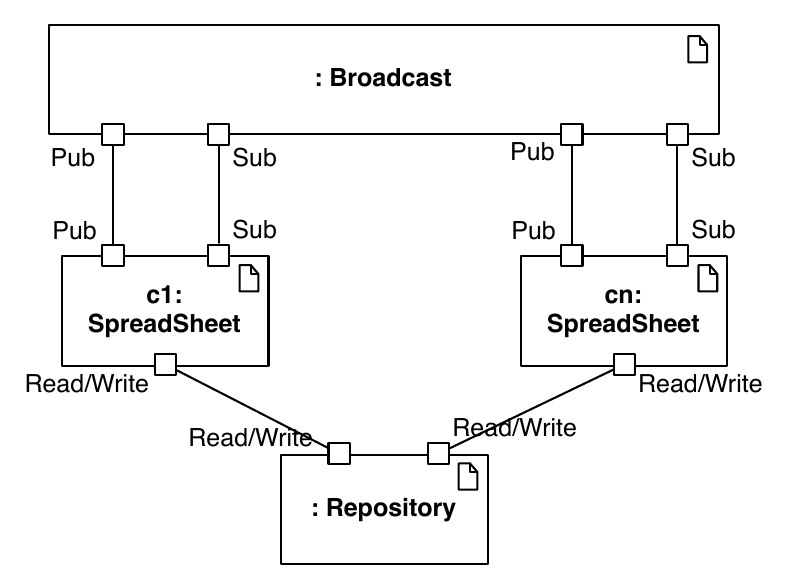
\includegraphics[width=80mm]{x-SocialCalc-cc}

    \optionA{The server implements the \textsc{: Repository} component and the \textsc{: Broadcast} connector.}
    \optionB{The server implements the \textsc{: Repository} component.}
    \optionC{The server implements the \textsc{: Broadcast} connector.}
    \optionD{The server implements the \textsc{SpreadSheet} components}
 \putOptions
\end{ClosedQuestion}
}

%15
\newcommand{\qSocialCalcParser}{
\begin{ClosedQuestion}
	Consider the architectural views for the SocialCalc system. The following diagram depicts a proposal for a component-and-connector view of the client Spreadsheet. A \textsc{Parser} module is used when loading a file
	
	\centering
	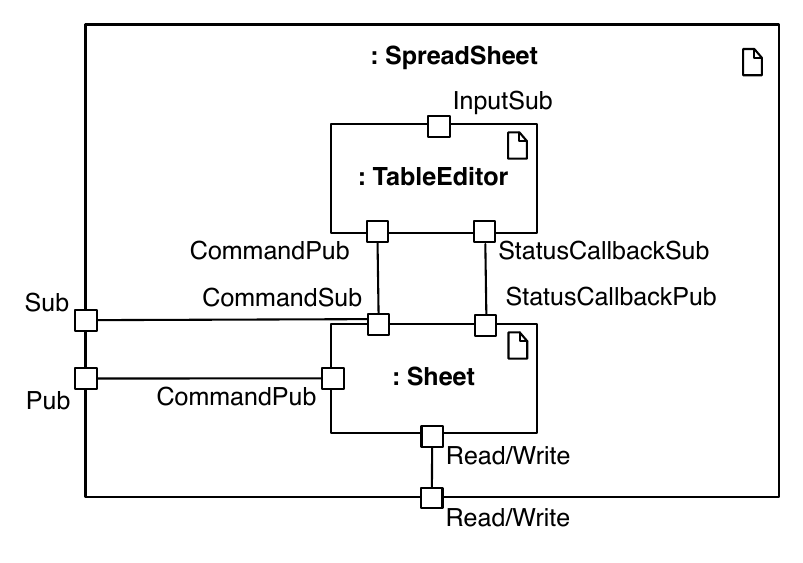
\includegraphics[width=80mm]{x-SocialCalc-cc-client}

    \optionA{The \textsc{Parser} module is part of the code executed by the \textsc{: TableEditor} component.}
    \optionB{The \textsc{Parser} module is part of the code executed by the \textsc{: Sheet} component.}
    \optionC{The code of the \textsc{Parser} module is executed by a repository component, which is not represented in the view.}
    \optionD{The code of the \textsc{Parser} module is executed by both, the \textsc{: Sheet} and the repository components (the latter is not visible in the view).}
 \putOptions
\end{ClosedQuestion}
}

%16
\newcommand{\qSocialCalcConflictResolution}{
\begin{ClosedQuestion}
	Consider the architectural views for the SocialCalc system. The following diagram depicts a proposal for a component-and-connector view of the client Spreadsheet. A \textsc{ConflictResolution} module is used when local commands conflict with remote commands.
	
	\centering
	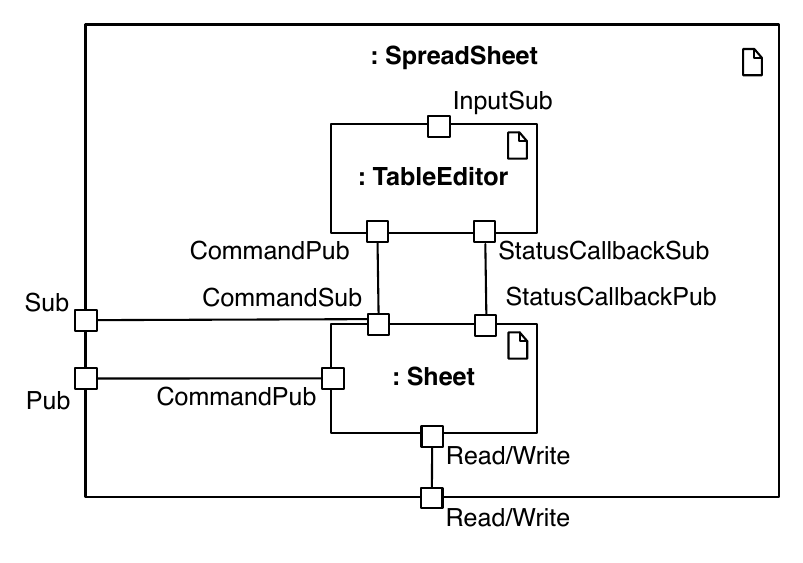
\includegraphics[width=80mm]{x-SocialCalc-cc-client}

    \optionA{The \textsc{ConflictResolution} module is part of the code executed by the \textsc{: TableEditor} component.}
    \optionB{The \textsc{ConflictResolution} module is part of the code executed by the \textsc{: Sheet} component.}
    \optionC{The code of the \textsc{ConflictResolution} module is executed by a broadcast connector that implements an eventbus between the \textsc{SpreadSheet} components.}
    \optionD{The code of the \textsc{ConflictResolution} module is executed in a server component because it needs to be centralized.}
 \putOptions
\end{ClosedQuestion}
}


% Domain Logic and Access Patterns

%17
\newcommand{\qLogicAccessDomainModel}{
\begin{ClosedQuestion}
	When the domain logic is organized using a Domain Model pattern the most suitable data source patterns are

    \optionA{Table Data Gateway and Row Data Gateway.}
    \optionB{Row Data Gateway and Active Record.}
    \optionC{Row Data Gateway and Data Mapper.}
    \optionD{Active Record and Data Mapper.}
 \putOptions
\end{ClosedQuestion}
}

%18
\newcommand{\qLogicAccessTransactionScript}{
\begin{ClosedQuestion}
	When the domain logic is organized using a Transaction Script pattern the most suitable data source patterns are

    \optionA{Table Data Gateway and Row Data Gateway.}
    \optionB{Row Data Gateway and Active Record.}
    \optionC{Row Data Gateway and Data Mapper.}
    \optionD{Active Record and Data Mapper.}
 \putOptions
\end{ClosedQuestion}
}

%19
\newcommand{\qLogicAccessTransactionScriptDomainObjects}{
\begin{ClosedQuestion}
	When the domain logic is organized using a Transaction Script pattern the domain objects

    \optionA{Are responsible for loading the objects they refer to.}
    \optionB{Are responsible for the management of transactions, begin and end of transactions.}
    \optionC{Contain the business logic.}
    \optionD{May not even exist, only record sets are used.}
 \putOptions
\end{ClosedQuestion}
}

%20
\newcommand{\qLogicAccessTableModule}{
\begin{ClosedQuestion}
	When the domain logic is organized using a Table Module pattern 

    \optionA{An object oriented style is followed.}
    \optionB{The business logic is organized around record sets.}
    \optionC{Row Data Gateway is the most suitable data source pattern.}
    \optionD{A Service Layer should be used to provide an interface for the presentation layer.}
 \putOptions
\end{ClosedQuestion}
}
